\documentclass[a4paper]{article}

\usepackage[UTF8]{ctex}
\usepackage[a4paper,margin=1in]{geometry}
\usepackage{graphicx}
\usepackage{float}
\usepackage{listings}
\usepackage{longtable}
\usepackage{booktabs}
\usepackage{hyperref}
\usepackage{fancyhdr}
\usepackage{lastpage}
\usepackage{color}
\usepackage{indentfirst}        % 首段缩进
\setlength{\parindent}{2em}     % 缩进2字符
\usepackage{zhnumber}           % 中文编号
\usepackage[dvipsnames]{xcolor}

%\newcommand{\college}{中山大学计算机学院}
\newcommand{\projname}{数据库系统原理实验| 实验2}
\newcommand{\reporttitle}{数据库系统原理实验二}
\newcommand{\stuno}{23336179}
\newcommand{\authorname}{马福泉}
\newcommand{\major}{计算机科学与技术}
\newcommand{\adviser}{赖韩江}
\newcommand{\startdate}{2025年9月25日}
\newcommand{\labenddate}{2025年9月26日}
\newcommand{\labroom}{B202}

\pagestyle{fancy} % 使用 fancyhdr 风格
\fancyhf{}      % 清空默认的页眉页脚

% 设置页眉
\fancyhead[L]{\kaishu \projname}      % 左侧页眉显示项目名称
\fancyhead[C]{\kaishu \reporttitle}    % 中间页眉显示报告标题
\fancyhead[R]{\kaishu \authorname} % 右侧页眉显示作者姓名

% 设置页脚
\fancyfoot[C]{第 \thepage 页，共 \pageref{LastPage} 页} % 中间页脚显示页码

% 去除页眉页脚与正文之间的分隔线
\renewcommand{\headrulewidth}{0.4pt}
\renewcommand{\footrulewidth}{0pt}

% 设置文档背景颜色
\definecolor{mybgcolor}{RGB}{0, 0, 0} % 定义背景颜色
\definecolor{NavyBlue}{RGB}{0,0,128} % 添加颜色定义
% \pagecolor{mybgcolor} % 设置背景颜色

% listing 配置rust
% \lstdefinelanguage{Rust}{
%   keywords={fn, let, mut, struct, enum, impl, pub, use, mod, trait, where},
%   keywordstyle=\color{NavyBlue},
%   comment=[l]{//},
%   commentstyle=\color{gray},
% }
% \lstset{language=Rust}

\lstset{
  basicstyle=\ttfamily\small,
  keywordstyle=\color{NavyBlue},
  commentstyle=\color{gray},
  stringstyle=\color{red},
  showstringspaces=false,
  extendedchars=false, % 关键：不处理中文
  breaklines=true
}

\begin{document}

% 封面
\begin{titlepage}
    \centering
    

    
\includegraphics[width=10cm]{img/SYSULogo.png}

    \vspace{1em}
    %{\Large \college \par}
    \vspace{1em}
    {\Large \kaishu \projname \par}
    \vspace{3em}

    

    
    {\fontsize{40pt}{42pt}\kaishu \selectfont \boldmath \reporttitle\par}
    \vspace*{\fill}

    \begin{center}
    {\Large
    \makebox[5em][s]{学号}:\underline{\makebox[15em][c]{\kaishu \stuno}}\\[1em]
    \makebox[5em][s]{姓名}:\underline{\makebox[15em][c]{\kaishu \authorname}}\\[1em]
    \makebox[5em][s]{专业}:\underline{\makebox[15em][c]{\kaishu \major}}\\[1em]
    \makebox[5em][s]{课程教师}:\underline{\makebox[15em][c]{\kaishu \adviser}}\\[1em]
    \makebox[5em][s]{起始日期}:\underline{\makebox[15em][c]{\kaishu \startdate}}\\[1em]
    \makebox[5em][s]{结束日期}:\underline{\makebox[15em][c]{\kaishu \labenddate}}\\[1em]
    \makebox[5em][s]{实验地点}:\underline{\makebox[15em][c]{\kaishu \labroom}}
    }
    \end{center}

    \vspace*{\fill}
\end{titlepage}

% 目录
\tableofcontents
\newpage


\section{实验概述}

\subsection{实验目的}

理解和掌握数据库DDL语言，能够熟悉地使用SQL DDL语句对数据库表进行增加、更新以及删除数据。

\subsection{实验内容}

向数据表中添加数据\\
图书借阅数据库系统JY”中数据表的内容如表1～表3所示。

\begin{table}[H]
\centering
\caption{图书表}
\label{tab:books}
\begin{tabular}{|p{1.2cm}|p{2.5cm}|p{2.5cm}|p{2.5cm}|p{2.5cm}|p{2.5cm}|p{2.5cm}|}
\hline
\textbf{book\_id} & \textbf{book\_name} & \textbf{book\_isbn} & \textbf{book\_author} & \textbf{book\_publisher} & \textbf{interviews\_times} & \textbf{book\_price} \\
\hline
b0001 & SQL Server 2012宝典 & 978-7-121-22013-5 & 廖梦怡 & 电子工业出版社 & 18 & 89.00 \\
\hline
b0002 & 职称英语专用教材 & 978-7-121-14800-2 & 孙若红 & 电子工业出版社 & 35 & 45.00 \\
\hline
b0003 & 中国通史 & 978-7-5388-53155 & 于海娣 & 黑龙江科学技术出版社 & 25 & 68.00 \\
\hline
b0004 & 丰子恺儿童文学选集 & 978-7-5007-8972-7 & 丰子恺 & 中国少年儿童出版社 & 40 & 22.50 \\
\hline
b0005 & 英语同义词辨析词典 & 978-7-5135-2294-6 & 赵同水 & 外语教学与研究出版社 & 6 & 55.00 \\
\hline
b0006 & 数据库基础与应用 & 978-7-304-06430-3 & 徐孝凯 & 中央广播电视大学出版社 & 5 & 35.00 \\
\hline
b0007 & 微积分初步 & 978-7-304-03742-0 & 赵坚 & 中央广播电视大学出版社 & 4 & 17.00 \\
\hline
b0008 & ASP.NET从入门到精通 & 978-7-302-28753-7 & 明日科技 & 清华大学出版社 & 27 & 89.80 \\
\hline
\end{tabular}
\end{table}
\begin{table}[H]
\centering
\caption{读者表}
\label{tab:readers}
\begin{tabular}{|c|c|c|c|}
\hline
\textbf{reader\_id} & \textbf{reader\_name} & \textbf{reader\_sex} & \textbf{reader\_department} \\
\hline
r0001 & 李德海 & 男 & 信息工程系 \\
\hline
r0002 & 柳承运 & 男 & 信息工程系 \\
\hline
r0003 & 安歌 & 女 & 涉外教育系 \\
\hline
r0004 & 谢嫣然 & 女 & 涉外教育系 \\
\hline
r0005 & 陈静玉 & 女 & 涉外教育系 \\
\hline
r0006 & 李媛媛 & 女 & 经济管理系 \\
\hline
r0007 & 胡锦波 & 男 & 经济管理系 \\
\hline
r0008 & 蔡明伟 & 男 & 行政管理系 \\
\hline
\end{tabular}
\end{table}
\begin{table}[H]
\centering
\caption{借阅记录表}
\label{tab:record}
\begin{tabular}{|c|c|c|c|c|}
\hline
\textbf{reader\_id} & \textbf{book\_id} & \textbf{borrow\_date} & \textbf{return\_date} & \textbf{notes} \\
\hline
r0001 & b0003 & 2014-01-12 & 2014-01-12 & NULL \\
\hline
r0001 & b0005 & 2014-01-26 & 2014-06-21 & NULL \\
\hline
r0004 & b0001 & 2014-03-02 & 2014-04-20 & NULL \\
\hline
r0004 & b0008 & 2014-03-26 & 2014-05-28 & NULL \\
\hline
r0006 & b0001 & 2014-04-16 & 2014-07-11 & NULL \\
\hline
r0007 & b0006 & 2014-05-08 & 2014-09-17 & NULL \\
\hline
r0008 & b0008 & 2014-06-29 & 2014-08-29 & NULL \\
\hline
r0008 & b0007 & 2014-08-15 & 2014-10-21 & NULL \\
\hline
\end{tabular}
\end{table}
具体实验内容：\\
1.向数据表中添加数据（数据表已创建）\\
2.删除借阅记录表 中 notes 的 not null 约束。\\
3.批量数据INSERT语句\\
3.1创建一个新的读者表2，把读者表中所有涉外教育系的读者插入到新的读者表2中；\\
3.2 创建一个借阅统计表，记录每位读者的借阅次数。如 (r0001, 2）。\\
4更新数据表中的数据\\
4.1将图书表book中interviews\_times列的值改为0\\
4.2更新图书表book中“电子工业出版社”的interviews\_times列值为10\\
4.3利用一个表的数据来修改另一个表的数据：将借阅记录表中的notes更新为图书表的book\_name。如\\
r0001 \& b0003 \& 2014-01-12 \& 2014-01-12 \& 中国通史\\
4.4借阅记录表中的notes全部设为NULL（空值）\\
5.删除数据表中的数据\\
5.1删除读者表reader中reader\_id为“r0003”的读者信息\\
5.2删除借阅记录表中行政管理系的学生的借阅数据 （r0008的借阅记录，即最后二行被删除）
\section{实验报告}

\subsection{实验步骤与结果}

\subsubsection{步骤1：向数据表中添加数据}

首先向图书表、读者表和借阅记录表中添加基础数据。由于数据表已创建，我们直接使用INSERT语句插入数据。

\textbf{1.1 向图书表插入数据}

\begin{lstlisting}[language=SQL, caption=向图书表插入数据]
INSERT INTO book VALUES 
('b0001', 'SQL Server 2012宝典', '978-7-121-22013-5', '廖梦怡', '电子工业出版社', 18, 89.00),
('b0002', '职称英语专用教材', '978-7-121-14800-2', '孙若红', '电子工业出版社', 35, 45.00),
('b0003', '中国通史', '978-7-5388-53155', '于海娣', '黑龙江科学技术出版社', 25, 68.00),
('b0004', '丰子恺儿童文学选集', '978-7-5007-8972-7', '丰子恺', '中国少年儿童出版社', 40, 22.50),
('b0005', '英语同义词辨析词典', '978-7-5135-2294-6', '赵同水', '外语教学与研究出版社', 6, 55.00),
('b0006', '数据库基础与应用', '978-7-304-06430-3', '徐孝凯', '中央广播电视大学出版社', 5, 35.00),
('b0007', '微积分初步', '978-7-304-03742-0', '赵坚', '中央广播电视大学出版社', 4, 17.00),
('b0008', 'ASP.NET从入门到精通', '978-7-302-28753-7', '明日科技', '清华大学出版社', 27, 89.80);
\end{lstlisting}

\textbf{1.2 向读者表插入数据}

\begin{lstlisting}[language=SQL, caption=向读者表插入数据]
INSERT INTO reader VALUES 
('r0001', '李德海', '男', '信息工程系'),
('r0002', '柳承运', '男', '信息工程系'),
('r0003', '安歌', '女', '涉外教育系'),
('r0004', '谢嫣然', '女', '涉外教育系'),
('r0005', '陈静玉', '女', '涉外教育系'),
('r0006', '李媛媛', '女', '经济管理系'),
('r0007', '胡锦波', '男', '经济管理系'),
('r0008', '蔡明伟', '男', '行政管理系');
\end{lstlisting}

\textbf{1.3 向借阅记录表插入数据}

\begin{lstlisting}[language=SQL, caption=向借阅记录表插入数据]
INSERT INTO record (reader_id, book_id, borrow_date, return_date, notes)
VALUES
('r0001','b0003','2014-01-12','2014-01-12',''),
('r0001','b0005','2014-01-26','2014-06-21',''),
('r0004','b0001','2014-03-02','2014-04-20',''),
('r0004','b0008','2014-03-26','2014-05-28',''),
('r0006','b0001','2014-04-16','2014-07-11',''),
('r0007','b0006','2014-05-08','2014-09-17',''),
('r0008','b0008','2014-06-29','2014-08-29',''),
('r0008','b0007','2014-08-15','2014-10-21','');
\end{lstlisting}

\begin{figure}[H]
\centering
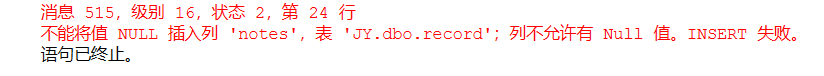
\includegraphics[width=0.8\textwidth]{img/error.png}
\caption{插入NULL出现错误}
\label{fig:error}
\end{figure}
由于notes列有NOT NULL约束，插入空字符串会报错。我们可以先插入空字符串，然后再删除NOT NULL约束。

\begin{figure}[H]
\centering
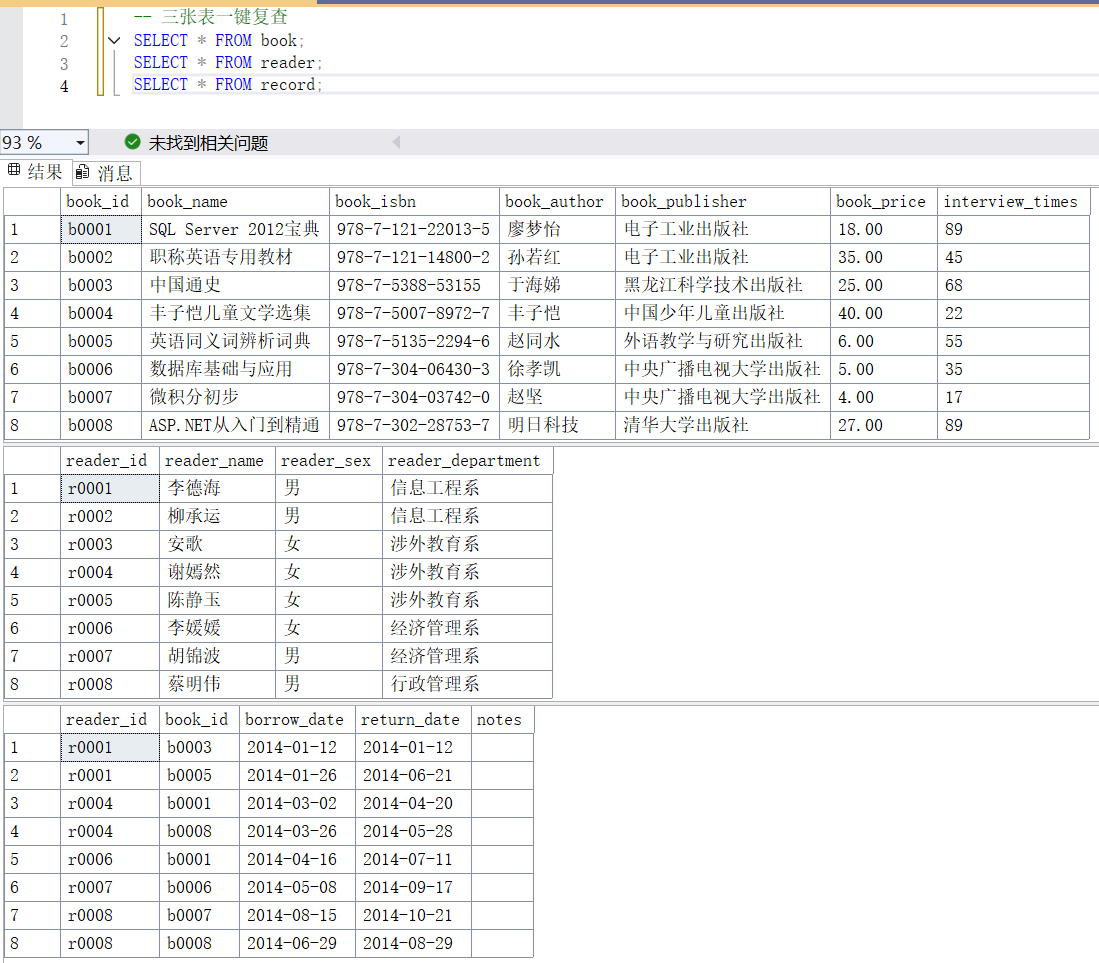
\includegraphics[width=0.8\textwidth]{img/insert_data_result.png}
\caption{数据插入结果}
\label{fig:insert_data}
\end{figure}

\subsubsection{步骤2：删除record表中notes列的NOT NULL约束}

\begin{lstlisting}[language=SQL, caption=删除NOT NULL约束]
ALTER TABLE record ALTER COLUMN notes VARCHAR(255) NULL;
\end{lstlisting}

\begin{figure}[H]
\centering
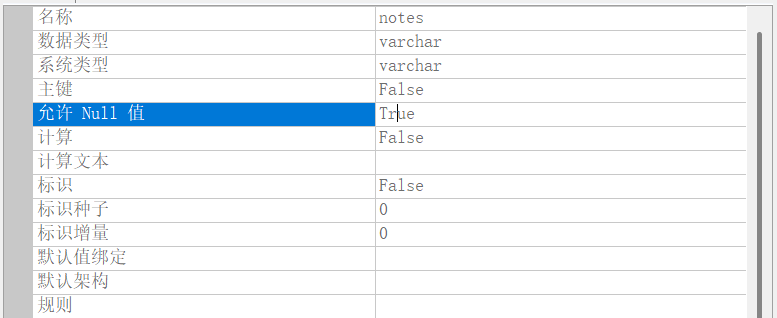
\includegraphics[width=0.8\textwidth]{img/alter_constraint_result_1.png}
\caption{删除约束结果}
\label{fig:alter_constraint1}
\end{figure}

\begin{figure}[H]
\centering
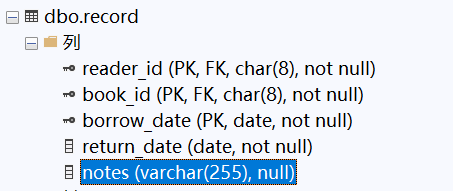
\includegraphics[width=0.8\textwidth]{img/alter_constraint_result_2.png}
\caption{删除约束结果}
\label{fig:alter_constraint2}
\end{figure}
如图，成功删除了NOT NULL约束。

\subsubsection{步骤3：批量数据INSERT语句}

\textbf{3.1 创建读者表2并插入涉外教育系的读者}

\begin{lstlisting}[language=SQL, caption=创建读者表2并插入数据]
-- 创建新的读者表2
CREATE TABLE reader2 (
    reader_id CHAR(5) PRIMARY KEY,
    reader_name VARCHAR(20) NOT NULL,
    reader_sex CHAR(2) CHECK (reader_sex IN ('男', '女')),
    reader_department VARCHAR(20) NOT NULL
);

-- 将涉外教育系的读者插入到读者表2中
INSERT INTO reader2 
SELECT reader_id, reader_name, reader_sex, reader_department 
FROM reader 
WHERE reader_department = '涉外教育系';
\end{lstlisting}

\begin{figure}[H]
\centering
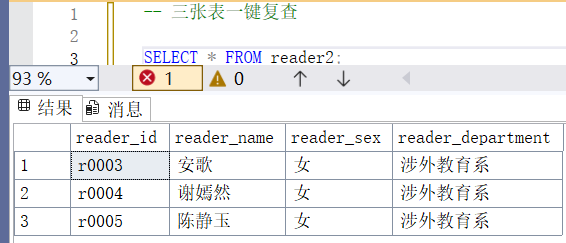
\includegraphics[width=0.8\textwidth]{img/reader2_result.png}
\caption{读者表2创建和数据插入结果}
\label{fig:reader2}
\end{figure}
如图，成功创建了读者表2并插入了涉外教育系的读者。

\textbf{3.2 创建借阅统计表}

\begin{lstlisting}[language=SQL, caption=创建借阅统计表]
-- 创建借阅统计表
CREATE TABLE borrow_statistics (
    reader_id CHAR(5) PRIMARY KEY,
    borrow_count INT NOT NULL DEFAULT 0
);

-- 插入每位读者的借阅次数统计
INSERT INTO borrow_statistics (reader_id, borrow_count)
SELECT reader_id, COUNT(*) as borrow_count
FROM record
GROUP BY reader_id;
\end{lstlisting}

\begin{figure}[H]
\centering
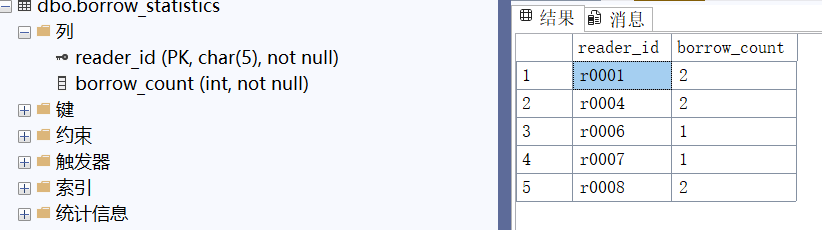
\includegraphics[width=0.8\textwidth]{img/borrow_statistics_result.png}
\caption{借阅统计表创建和数据插入结果}
\label{fig:borrow_statistics}
\end{figure}
如图，成功创建了借阅统计表并插入了每位读者的借阅次数。


\subsubsection{步骤4：更新数据表中的数据}

\textbf{4.1 将图书表中interviews\_times列的值改为0}

\begin{lstlisting}[language=SQL, caption=更新interviews\_times为0]
UPDATE book SET interviews_times = 0;
\end{lstlisting}

\begin{figure}[H]
\centering
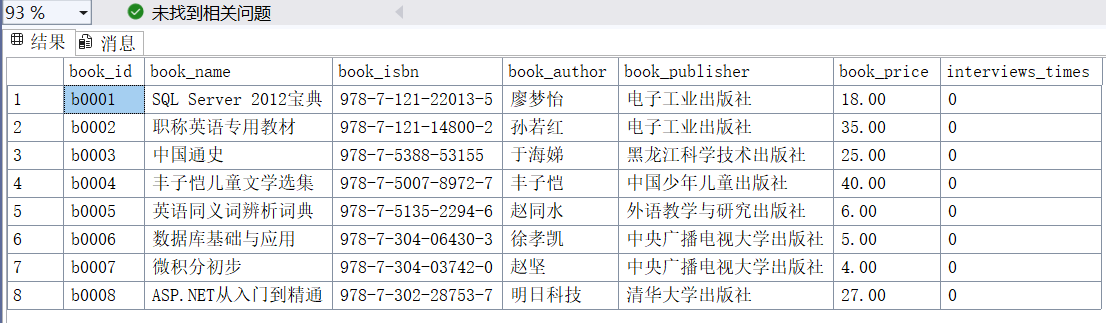
\includegraphics[width=0.8\textwidth]{img/update_interviews_times_zero.png}
\caption{更新interviews\_times为0的结果}
\label{fig:update_zero}
\end{figure}
如图，成功将interviews\_times列的值更新为0。


\textbf{4.2 更新电子工业出版社的interviews\_times为10}

\begin{lstlisting}[language=SQL, caption=更新电子工业出版社的interviews\_times]
UPDATE book 
SET interviews_times = 10 
WHERE book_publisher = '电子工业出版社';
\end{lstlisting}

\begin{figure}[H]
\centering
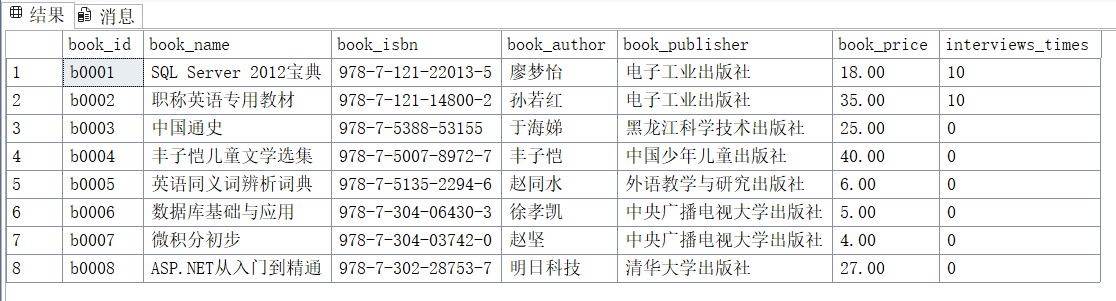
\includegraphics[width=0.8\textwidth]{img/update_publisher_interviews.png}
\caption{更新电子工业出版社interviews\_times的结果}
\label{fig:update_publisher}
\end{figure}
如图，成功将电子工业出版社的interviews\_times列值更新为10。


\textbf{4.3 用图书表的book\_name更新借阅记录表的notes}

\begin{lstlisting}[language=SQL, caption=更新借阅记录表的notes为书名]
UPDATE record 
SET notes = (
    SELECT book_name 
    FROM book 
    WHERE book.book_id = record.book_id
);
\end{lstlisting}

\begin{figure}[H]
\centering
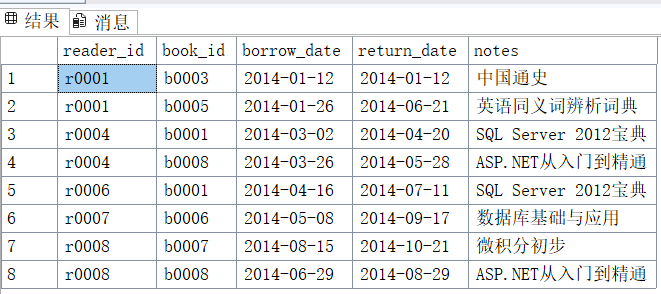
\includegraphics[width=0.8\textwidth]{img/update_notes_bookname.png}
\caption{更新notes为书名的结果}
\label{fig:update_notes}
\end{figure}
如图，成功将借阅记录表的notes列更新为对应的书名。


\textbf{4.4 将借阅记录表中的notes全部设为NULL}

\begin{lstlisting}[language=SQL, caption=将notes设为NULL]
UPDATE record SET notes = NULL;
\end{lstlisting}

\begin{figure}[H]
\centering
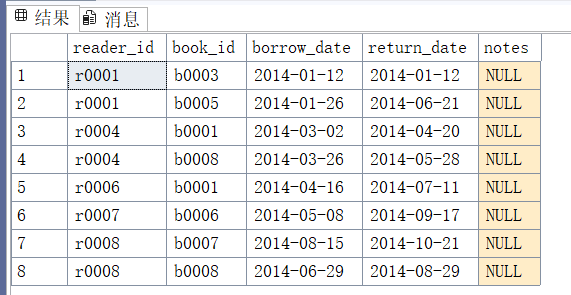
\includegraphics[width=0.8\textwidth]{img/update_notes_null.png}
\caption{将notes设为NULL的结果}
\label{fig:update_null}
\end{figure}
如图，成功将借阅记录表的notes列全部设为NULL。


\subsubsection{步骤5：删除数据表中的数据}

\textbf{5.1 删除reader\_id为"r0003"的读者信息}

\begin{lstlisting}[language=SQL, caption=删除特定读者信息]
DELETE FROM reader WHERE reader_id = 'r0003';
\end{lstlisting}

\begin{figure}[H]
\centering
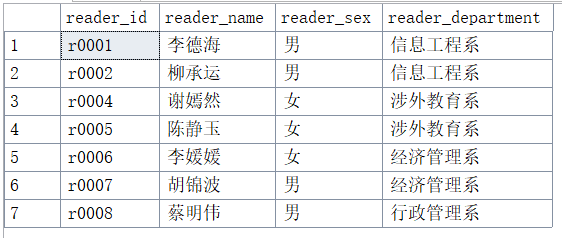
\includegraphics[width=0.8\textwidth]{img/delete_reader_r0003.png}
\caption{删除读者r0003的结果}
\label{fig:delete_reader}
\end{figure}
如图，成功删除了reader\_id为"r0003"的读者信息。

\textbf{5.2 删除行政管理系学生的借阅记录}

\begin{lstlisting}[language=SQL, caption=删除行政管理系学生的借阅记录]
DELETE FROM record 
WHERE reader_id IN (
    SELECT reader_id 
    FROM reader 
    WHERE reader_department = '行政管理系'
);
\end{lstlisting}

\begin{figure}[H]
\centering
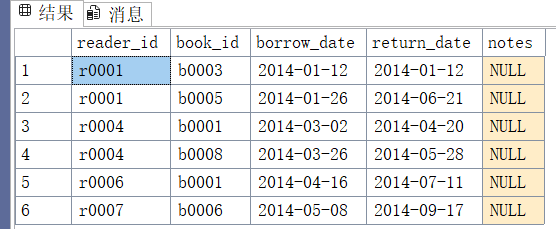
\includegraphics[width=0.8\textwidth]{img/delete_admin_record.png}
\caption{删除行政管理系学生借阅记录的结果}
\label{fig:delete_admin}
\end{figure}
如图，成功删除了行政管理系学生（读者r0008）的借阅记录。

\subsection{实验总结}

通过本次实验，我初步掌握了以下SQL DDL和DML操作：

\begin{enumerate}
    \item \textbf{数据插入（INSERT）}：学会了使用INSERT语句向表中添加单条和多条记录，包括VALUES和SELECT子查询两种方式。
    \item \textbf{表结构修改（ALTER）}：掌握了使用ALTER TABLE语句修改表结构，包括修改列约束等操作。
    \item \textbf{数据更新（UPDATE）}：熟练运用UPDATE语句更新表中的数据，包括简单更新、条件更新和使用子查询更新等多种方式。
    \item \textbf{数据删除（DELETE）}：学会了使用DELETE语句删除表中的数据，包括简单删除和使用子查询进行条件删除。
    \item \textbf{统计查询}：通过GROUP BY和COUNT函数实现了数据统计功能。
\end{enumerate}

本次实验加深了我对数据库操作的理解，特别是在数据操作语言（DML）方面的应用。同时，通过创建新表和数据迁移的操作，也提升了我对数据库设计和管理的认识。

\textbf{易错点总结：}
\begin{itemize}
    \item \textbf{NOT NULL约束未解除时插入NULL或空字符串会报错}，需先修改表结构再插入或更新数据。
    \item \textbf{UPDATE带子查询时要确保子查询只返回一行}，否则会报“子查询返回多于一行”错误。
    \item \textbf{DELETE语句中使用IN子查询时}，要确保子查询结果与主表字段类型一致。
    \item \textbf{表名、字段名变更后需同步修改所有相关SQL语句}，否则会出现“对象不存在”或“列名无效”错误。
    \item \textbf{插入中文数据时注意字符集和编码问题}，避免乱码或插入失败。
    \item \textbf{批量插入或更新时注意主键、唯一约束冲突}，否则会导致插入失败。
\end{itemize}

\end{document}